\chapter{Сравнительный анализ решений}

\section{Протокол H.323}

\subsection{Краткое описание протокола}

Протокол H.323~"--- рекомендация сектора стандартизации электросвязи МСЭ (\foreigne{International Telecommunication Union -- Telecommunication sector, ITU-T}).
Этот стандарт не~связан с~протоколом IP, но~большинство его реализаций сделано основе этого протокола (см. рис. \ref{fig:H232stack}).

\begin{figure}
    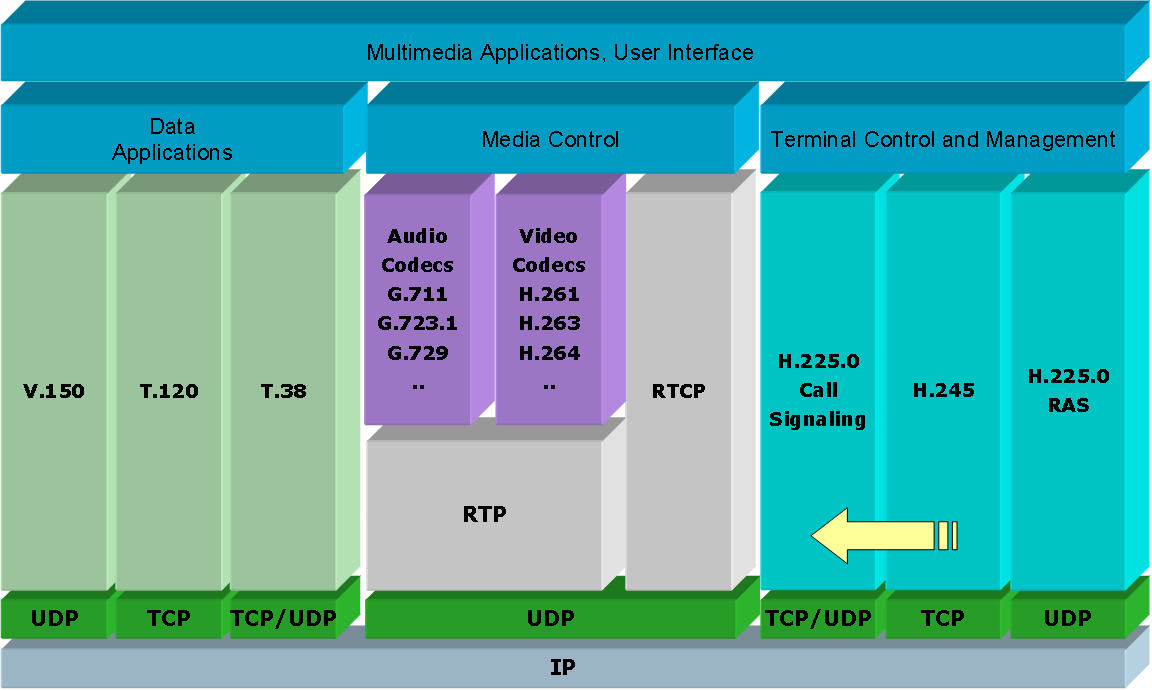
\includegraphics[width = \columnwidth]{figures/H323Stack.png}
    \caption{Полный стек протоколов H.323 на~базе протокола IP}
    \label{fig:H232stack}
\end{figure}

H.323 разделяет передачу данных на~4 составляющие:\listnopagebreak
\begin{enumerate}
    \itemсигнализация~"--- формирование соединения и~управление его статусом;
		\itemуправление потоковым мультимедиа~"--- передача данных посредством~транспортных протоколов реального времени (RTP);
		\itemприложения передачи данных~"--- передача в~рамках соответствующих стандартов, таких как~T.120 и~T.38;
		\itemкоммуникационные интерфейсы~"--- взаимодействие устройств на~физическом, канальном, сетевом уровнях.
\end{enumerate}

Устройства, описываемые протоколом H.323, разделяются на~следующие типы:\listnopagebreak
\begin{itemize}
    \item\keyworde{терминалы}{terminals};
		\item\keyworde{шлюзы}{gateways};
		\item\keyworde{привратники}{gatekeepers};
		\item\keyworde{сервера многосторонней конференции}{multipoint control unit, MCU}.
\end{itemize}

\paragraph{Терминал.} Терминал~"--- компьютер или~любое другое автономное устройство, способное выполнять мультимедийное приложение с~поддержкой звуковой связи, и, если~необходимо, обладающее возможностью передачи данных или~видео.

Терминал должен поддерживать протоколы:\listnopagebreak
\begin{itemize}
    \item\ H.245~"--- cогласование параметров соединения;
    \item\ Q.931~"--- установление и~контроль соединения;
    \item\ RAS~"--- взаимодействие с~привратником;
    \item\ RTP/RTCP~"--- оптимизация доставки потокового аудио/видео;
    \item\ G.711~"--- кодек для~передачи звуковой информации;
    \item\ семейство протоколов H.450~"--- для~поддержки обязательных в~H.323 дополнительных видов обслуживания.
\end{itemize}

Основная функция терминала~"--- обеспечение двухсторонней речевой или~мультимедийной связи с~другим терминалом, шлюзом или~устройством управления конференцией.

\paragraph{Шлюз.} Шлюз необходим для~установления соединения с~терминалом другого стандарта.
Связь между~терминалами различных стандартов осуществляется за~счёт трансляции протоколов установки соединений, передачи данных и~разрыва соединений.
Шлюзы не~являются необходимыми компонентами сети по~протоколу H.323, но, тем не~менее, они~широко применяются для~сочленения сетей IP-телефонии с~коммутируемыми цифровыми или~аналоговыми телефонными сетями.

\paragraph{Привратник.} Привратник, или~контроллер зоны H.323~"--- устройство или~программа, выполняющие важнейшие функции управления вызовами.
Под~\keyword{зоной} подразумевается совокупность всех устройств (терминалов, шлюзов и~MCU), находящихся под~управлением контроллера.
Внутри~одной сети может находиться несколько взаимодействующих привратников, и, как~следствие, несколько зон.

Основные функции привратника:\listnopagebreak
\begin{itemize}
    \itemтрансляция адресов ЛВС и~телефнных номеров в~адреса протокола IP;
		\itemуправление доступом, авторизация доступа в~сеть по~протоколу RAS;
		\itemуправление полосой пропускания;
		\itemмаршрутизация сигнальных сообщений между~терминалами внутри~зоны.
\end{itemize}

Наличие привратника в~сети не~является обязательным, если~вызывающий абонент знает IP-адрес терминала вызываемого абонента \citebook{solomonovich2006ip}, но~подобная схема существенно ограничивает мобильность пользователя.

\paragraph{MCU.} Сервер многоточечной конференции~"--- устройство, обеспечивающее конференц-связь двух или~более терминалов.
Рекомендация H.323 подразумевает три вида конференций:
\begin{enumerate}
    \item\keyword{Централизованные конференции}, в~которых обмен всеми данными проходит через~MCU по~схеме <<точка-точка>>.
    \item\keyword{Децентрализованные конференции}, использующие групповую адресацию; MCU лишь~передаёт контрольную и~управляющую информацию.
    \item\keyword{Гибридные конференции}~"--- используются оба подхода одновременно.
\end{enumerate}

\subsection{Реализации Н.323}

Все компоненты сети H.323 могут быть исполнены как~в программном виде, так~и в~аппаратно-программном~"--- специально спроектированном оборудовании.
Аппаратно-программное исполнение необходимо для~больших сетей IP-телефонии; оборудование, предоставляющее соединение по~протоколу H.323, производят все крупнейшие игроки отрасли: Ericsson, Tedas, Lucent Technologies, Siemens, Сisco, Avaya, Huawei, D-Link.

Из~программных решений, которые можно устанавливать и~на компьютеры общего пользования, что~бывает единственно возможным для~небольших предприятий, необходимо отметить наличие свободной реализации протокола H.323~"--- H323Plus, распространяемой по~лицензии Mozilla Public~License \citeonline{h323plus}, на~базе которой работают многие популярные проекты: Ekiga, Asterisk, FreeSwitch.

\section{Протокол SIP}

\subsection{Краткое описание протокола}

\keyworde{Протокол инициирования сеансов}{Session Initiation Protocol, SIP}~"--- популярный протокол IP-телефонии, разработанный группой Multiparty Multimedia Session Control (MMUSIC) Инженерного совета Интернета (\foreigne{Internet Engineering Task Force, IETF}).
В~основу протокола были заложены следующие принципы:\listnopagebreak
\begin{itemize}
    \itemпростота;
		\itemнезависимость от~транспортного уровня;
		\itemперсональная мобильность пользователей;
		\itemмасштабируемость сети;
		\itemрасширяемость протокола;
		\itemинтеграция в~стек существующих протоколов Интернета;
		\itemвзаимодействие с~другими протоколами сигнализации.
\end{itemize}

Несмотря на~то, что~в качестве транспортного протокола могут использоваться X.25, Frame Relay, IPX, AAL5/ATM \etc, предпочтительным является стек протоколов IP, TCP (порт 5060) и~UDP.

Протокол SIP имеет клиент-серверную архитектуру: клиент выдаёт запросы, которые обрабатываются на~сервере.
Непосредственно с~клиентом работают \keyworde{пользовательский агентский клиент}{User Agent Client, UAC} и~\keyworde{пользовательский агентский сервер}{UAS}.
При~наличии и~UAC, и~UAS имеет смысл говорить о~\keyworde{пользовательском агенте}{User Agent, UA}, который по~сути представляет собой терминальное оборудование.
Пользователь непосредственно работает только~с терминальным оборудованием.

Сервера протокола SIP делятся по~функциям на~следующие типы:
\begin{itemize}
    \itemпрокси-сервер;
		\itemсервер переадресации;
		\itemсервер определения местоположения пользователей;
		\itemсервер B2BUA.
\end{itemize}

\keyword{Прокси-сервер} представляет интересы пользователя в~сети.
Он~не~имеет права изменять структуру и~содержимое передаваемых сообщений, добавляет лишь~свою адресную информацию в~специальное поле <<Via>>.
Существуют два типа серверов: с~сохранением состояний и~без.
Первый тип может предоставить большое количество услуг: использование протокола TCP для~сигнальной информации, размножение запросов, многоадресная рассылка сигнальной информации; но~он работает медленее, чем~сервер второго типа, который работает только~как ретранслятор.

\keyword{Сервер переадресации} используется для~определения текущего местоположения пользователя.
Он~сообщает адрес либо~вызываемого пользователя, либо~прокси-сервера, по~которому инициатор запроса отправляет новый запрос, таким образом, сервер переадресации не~содержит клиентскую часть ПО.
Аналогично H.323, он~может не~использоваться, если~пользователь сам знает текущий адрес вызываемого абонента, что~точно так~же ограничивает мобильность, которая является одним из~принципов SIP.

Как~было замечено выше, мобильность пользователя является одним из~основных принципов SIP, поэтому необходимо определять текущее местоположение пользователя для~доставки ему сообщений и~передавать его серверу переадресации.
Для~этого текущий адрес пользователя хранится на~\keyword{сервере определения местоположения пользователей}.
Пользователь обязан проинформировать этот сервер при~подключении к~сети с~помощью команды <<REGISTER>>.
Часто этот сервер совмещён с~прокси-сервером, такой сервер носит название \keyword{registrar}.

\keyworde{Сервер спина-к-спине}{back-to-back user agent}~"--- разновидность прокси-сервера, работающая с~двумя и~более терминалами, разделяя вызов или~сеанс на~разные участки.
С~каждым участком B2BUA работает индивидуально, как~UAS по~отношению к~инициатору и~как UAC по~отношению к~принимающему вызов терминалу.
Сигнальные сообщения передаются в~рамках сеанса в~обе стороны синхронно.
Каждый из~участников соединения на~уровне сигнализации взаимодействует с~B2BUA, как~с оконечным устройством, хотя~в действительности сервер является посредником, который может использоваться для~следующих целей:
\begin{itemize}
    \itemбиллинг;
		\itemперевод звонка;
		\itemавтоматическое разъединение;
		\itemсопряжение сетей, в~т.\,ч. с~разными диалектами протокола;
		\itemсокрытия структуры сетей;
		\itemконтроль потоков данных внутри~сессии;
		\item\etc
\end{itemize}

В~первоначальной версии протокола SIP было всего 6~запросов: INVITE, ACK, BYE, CANCEL, REGISTER и~OPTIONS, что~соответствовало принципу простоты, заложенному в~основание протокола, но~в дальнейшем пришлось поддержать и~8~новых типов запросов.
Тем не~менее, даже~с увеличенным числом запросов~б\'{о}льшая их стуктурированность создаёт преимущество для~разработчиков относительно~протокола H.323 \citebook{meggelen2009asterisk}.
Более того, структура ответов на~запросы унаследована от~протокола HTTP, например, код 404 так~же соответствует ошибке <<Not Found>>; это упрощает разработку.

Протокол SIP определяет адресацию пользователей.
Адрес SIP подобен адресу электронной почты: первая часть идентифицирует пользователя, вторая часть~"--- домен сети, хоста или~IP-адрес, части разделяются знаком <<@>>.
Аналогично e-mail, идентификаторы алфавитно-цифровые, что~позволяет как~интегрировать SIP-системы с~системами электронной почты, так~и с~системами ТфОП, используя телефонный номер или~его часть как~идентификатор.

\subsection{Реализации SIP}

Благодаря~простоте протокола, существует очень много его программных реализаций, как~программ-клиентов, так~и серверов, поэтому мы~не будем перечислять основные реализации.
Программы-клиенты SIP доступны практически для~каждой платформы, включая мобильные и~платформы на~основе web-технологий.
Весьма часто программное обеспечение для~SIP имеет так~же и~функции протокола H.323, что~достигается схожестью интерфейсов протоколов для~конечного пользователя.

\section{Сравнение протоколов SIP и~H.323}

Два протокола, хотя~и решают одинаковую задачу, используют разные основы и~принципы.
Протокол H.323, более старый, был создан специалистами в~области традиционной телефонии, и~оказался ближе к~ТфОП.
Более молодой стандарт SIP создавался уже с~оглядкой на~распространение Интернета, поэтому большинство принципов его разработчики переняли оттуда.
Поэтому протокол SIP оказался предпочтительнее для~операторов, стремящихся к~технической интеграции своих услуг.

Поскольку~протоколы развивались параллельно, стремясь удовлетворить одинаковые потребности рынка, то на~данный момент существенного различия в~услугах нет.
Наиболее сильные отличия, тем не~менее, сохраняются в~организации конференций, так~как протокол H.323 предлагает более сложное решение с~обязательным использованием контроллера конференций MCU.
С~другой стороны, централизованность протокола H.323 предоставляет больше возможностей контроля над~конференциями.
Расширенные возможности контроля протокола H.323 проялвются и~в других областях, как, например, аутентификации и~учёта пользователей, контроль над~ресурсами.
Здесь возможности протокола SIP ограничены.

Наиболее сильные различия между~протоколами заключаются в~наборе дополнительных услуг.
Здесь стоит отметить преимущество протокола SIP, предоставляющем возможность организации связи третьей стороной, что~может использоваться секретарями и~операторами call-center; возможность задания приоритетов в~обслуживании вызовов; улучшенная поддержка мобильности пользователей.

Другим немаловажным преимуществом протокола SIP является его расширяемость, которая во~многом есть следствие простоты.
Неподдерживаемые запросы просто игнорируются серверами, использующими более старую версию протокола SIP, что~обеспечивает хорошую и~обратную совместимость и~прямую.
Расшифровка сообщений протокола H.323 более сложна, и~поэтому производители часто ограничиваются поддержкой только~одной версией протокола, что~может приводить к~несовместимости оборудования, предоставляемого разными производителями.
Добавление новой функциональности в~протокол H.323 может привести к~существенному изменению всех протоколов, и, как~следствие, их реализаций; протокол SIP~же обладает модульной структурой, модули могут быть изменены независимо друг от~друга.
SIP не~стандартизует кодеки, поэтому в~нём не~вызывает проблем использование приложений с~нестандартными алгоритмами кодирования.

Масштабируемость сетей на~базе протокола H.323 оказывается сильно ограниченной зональной структурой~"--- для~каждой новой зоны необходима установка нового привратника, пропускная способность которого меньше пропускной способности сервера SIP, которому не~нужно сохранять запросы.
С~другой стороны, из-за~отсутствия сохранения сведений о~запросах протокол SIP менее приспособлен к~интеграции с~ТфОП.

Время установления соединения является немаловажным фактором, определяющим привлекательность услуги IP-телефонии для~клиентов.
Упрощённость запросов протокола SIP позволяет существенно сократить время установления соединения по~сравнению с~протоколом H.323: SIP использует один запрос, в~то время как~H.323 производит многократный обмен сообщениями, который хотя~и можно сократить при~помощи некоторых техник, всё равно остаётся~б\'{о}льшим.

Как~уже было отмечено выше, протокол SIP использует HTTP-подобный текстовый формат сообщений, благодаря~чему анализ его работы проще для~программиста, так~как не~приходится использовать дешифратор, как~например в~протоколе H.323, использующем язык ASN.1.
С~другой стороны, обработка сообщений в~двоичном коде осуществляется быстрее, но~с увеличением вычислительных мощностей это преимущество теряется.

С~точки зрения пользователя использование обоих протоколов одинаково; существует, как~уже было отмечено, множество гибридных программ-клиентов, предоставляющих одинаковых графический интерфейс для~протоколов SIP и~H.323.
Таким образом, полнота принятия решений возлагается на~владельца сети, предоставляющей услуги.
Исходя из~вышесказанного следует, что~компании, пришедшие на~рынок IP-телефонии из~области интернет-услуг, выбирают протокол SIP, поскольку~он предоставляет большой спектр услуг, а~затраты на~подготовку кадров оказываются небольшими.
Компании, ранее предоставлявшие услуги обычной телефонии и~передачи данных, чаще выбирают протокол H.323, так~как он~более совместим с~традиционной телефонией, а~больший бюджет позволяет использовать и~новое оборудование, и~кадры.

\section{Другие решения}

Протоколы H.323 и~SIP, несмотря на~свою распространённость, не~являются единственными решениями для~IP-телефонии.

\subsection{Протокол MGCP}

\keyworde{Протокол управления транспортным шлюзами}{Media Gateway Control Protocol, MGCP}~"--- протокол, в~основе которого лежит идея декомпозиции шлюза на:
\begin{enumerate}
    \itemтранспортный шлюз, выполняющий функции преобразования речевой информации ТфОП в~пригодный для~передачи по~сетям IP вид и~обратно;
		\itemустройств управления шлюзом;
		\itemшлюз сигнализации, обеспечивающий обмен сигнальной информацией между~ТфОП и~устройством управления шлюзом.
\end{enumerate}

За~счёт такой декомпозиции достигается значительное уменьшение нагрузки на~процессора шлюзов, и, как~следствие, удешевление сети и~возможность простого масштабирования.
Б\'{о}льшая прозрачность в~соединении с~ТфОП делает этот протокол конкурентным с~H.323, в~частности, именно MGCP активно внедряется крупным производителем Nortel Networks;
хотя~крупным препятствием остаётся широкое использование H.323 в~существующих сетях IP-телефонии.

Недостатком стандарта MGCP является его незаконченность, вследствие~которой оборудование различных производителей становится несовместимым.
Не~определяет стандарт и~работу с~терминальными устройствами, стандартом \emph{de facto} является использование отдельного сервера или~привратника SIP.

\subsection{Skype}

\keyword{Skype}~"--- популярное программное средство IP-телефонии.
Работа этой программы основана на~принципах \keyworde{точка-точка}{point to point, P2P}, \ie~отказа от~дорогих централизованных серверов.
Передача данных между~двумя пользователями маршрутизируется через~компьютеры других пользователей, что~позволяет соединяться друг с~другом пользователям локальной сети без~передачи данных наружу.
Единственным централизованным узлом является сервер идентификации, на~котором хранятся учётные записи пользователей сети.

Очевидными преимуществами технологии Skype является мобильность (клиент есть практически под~все современные платформы), высокая скорость соединения за~счёт более оптимальной маршрутизации.
Тем не~менее, эта технология обладает и~рядом существенных недостатков.
Исходный код программы закрыт, что~автоматически вызывает вопросы о~конфиденциальности разговоров; также~невозможно ограничить работу Skype пределами одной локальной сети предприятия.
Корректная работа протокола типа P2P требует достаточно большого количества подключённых пользователей, в~случае массового сбоя программного обеспечения это число стихийно уменьшается и~разговор может стать невозможным.
Но~несмотря на~эти недостатки, Skype популярен как~у индивидуальных пользователей, так~и у~корпоративных, особенно~у компаний с~высокой мобильностью сотрудников.